\chapter{Other Eigenvalue Algorithms}

There is more to the computation of eigenvalues than the QR algorithm. In this chapter, we briefly mention three famous alternatives for real symmetric eigenvalue problems: the Jacobi algorithm, for full matrices, and the bisection and divide-and-conquer algorithms, for tridiagonal matrices.

\section{Jacobi} 
One of the oldest ideas for computing eigenvalues of matrices is the Jacobi algorithm, introduced by Jacobi in 1845. This method has attracted attention throughout the computer era, especially since the advent of parallel computing, though it has never quite managed to displace the competition.   

The idea is to diagonalize a small submatrix of $A$, then another, and so on, hoping eventually to converge to a diagonalization of the full matrix. 

We start with a $ 2\times 2 $ real symmetric matrix and its diagonalization: 

\begin{equation}
\label{eq: 2x2 diagonal jacobi}
    J^\top \begin{bmatrix}[] 
        a &  d \\
        d &  b \\
    \end{bmatrix} J = \begin{bmatrix}[] 
        \neq 0 &  0 \\
        0 &  \neq 0  \\
    \end{bmatrix}  
\end{equation}
where $J$ is orthogonal. Now there are several ways to choose $J$. One is the Householder reflection: 
\begin{equation}
\label{eq: 2x2 householder}
    F = \begin{bmatrix}[] 
        -c &  s \\
        s &  c \\
    \end{bmatrix}, 
\end{equation}
where $s=\sin \theta $ and $c=\cos \theta $ for $\theta $. Note that $\det F = -1$. Alternatively, one can use a rotation but not a reflection, 
\begin{equation}
\label{eq: 2x2 rotation}
    J = \begin{bmatrix}[] 
        c &  s \\
        -s &  c \\
    \end{bmatrix}, 
\end{equation}
with $\det J = 1$. This is the standard approach for the Jacobi algorithm. It can be shown that the diagonalization is accomplished if $\theta $ satisfies 
\begin{equation}
\label{eq: 2x2 condition}
    \tan(2 \theta ) = \frac{2d}{b-a}, 
\end{equation}
and the matrix $J$ based this choice is called a \textbf{Jacobi rotation}. Note that it has the same form as a Givens rotation, the only difference is that $\theta $ is chosen to make $J^\top A J$ diagonal rather than $ J^T A $ triangular. 

Now let $ A\in \RR^{m \times  m} $ be symmetric. The Jacobi algorithm of the iterative application of transformations \eqref{eq: 2x2 diagonal jacobi} based on matrices defined by \eqref{eq: 2x2 rotation} and \eqref{eq: 2x2 condition}. The matrix $J$ is now enlarged to an $ m\times m $ matrix that is the identity in all but four entries, where it has the form \eqref{eq: 2x2 rotation}. Applying $ J^\top  $ on the left modifies two rows of $ A $, and applying $ J $ on the right modifies two columns. At each step a symmetric pair of zeros is introduced into the matrix, but previous zeros are destroyed. Just as with the QR algorithm, however, the usual effect is that the magnitudes of these nonzeros shrink steadily. 

The approach naturally fitted to hand computation is to pick the largest off-diagonal entry at each step. We can show that $ \sum_{i\neq j} a_{ij}^{2}  $ decreases by at least the factor $ 1 - \frac{2}{m^{2} -m} $ at each step. After $ O(m^2) $ steps, each requiring $ O(m) $ operations, the sum of squares must drop by a constant factor, and convergence to accuracy $ \mep $ is assured after $ O(m^3\log (\mep))$ operations. In fact, it's known that the convergence is better than this, ultimately quadratic rather than linear, so the actual operation count is $ O\left( m^3 \log( |\log (\mep)|) \right)  $.

On a computer, the off-diagonal entries are generally eliminated in a cyclic manner that avoids the $ O(m^2) $ search for the largest. For example, if the $ m(m-1)/2 $ superdiagonal entries are eliminated in the simplest row-wise order, beginning with $ a_{12}, a_{13},\ldots, $ then rapid asymptotic convergence is again guaranteed. After one {\it sweep} of $ 2\times 2 $ operations involving all of them $ \frac{(m-1)}{2} $ pairs of off-diagonal entries, the accuracy has generally improved by better than a constant factor, and again, the convergence is ultimately quadratic.   


%────────────────────────────────────────
\begin{note}

The Jacobi method is attractive because it deals only with pairs of rows and columns at a time, making it easily parallelizable. The matrix is not tridiagonalized in advance; the Jacobi rotations would destroy that structure. Convergence for matrices of dimension $ m\le 1000 $ is typically achieved in fewer than ten sweeps, and the final componentwise accuracy is generally even better than can be achieved by the QR algorithm. Unfortunately, even on parallel machines, the Jacobi algorithm is not usually as fast as tridiagonalization followed by the QR or divide-and-conquer algorithm, though it usually comes within a factor of $ 10 $. 
\end{note}
%────────────────────────────────────────

\section{Bisection}
After a symmetric matrix has been tridiagonalized, this is the standard next step of one does not want all of the eigenvalues but just a subset of them.  For example, bisection can find the largest $ 10\% $ of the eigenvalues, or the smallest thirty eigenvalues, or all the eigenvalues in the in the interval $ [1,2] $.  Once the desired eigenvalues are found, the corresponding eigenvectors can bee obtained by one step of inverse iteration (Algo~\ref{Algo 27.2}). 

Since the eigenvalues of a real symmetric matrix are real, we can find them by searching the real line for roots of the polynomial $ p(x) =\det(A-xI) $. This sounds like a bad idea, for did we not mention in Chapter 14 and 24 that polynomial rootfinding is highly unstable procedure for finding eigenvalues? The difference is that those remarks pertained to the idea of find roots from the polynomial {\it coefficients}.  Now, the idea is to find the roots by evaluating $ p(x) $ at various points $ x $, without ever looking at its coefficients, and applying the usual bisection process for nonlinear functions. This could be done, for example, by Gaussian elimination with pivoting, and the resulting algorithm would be highly stable.  

This much sounds useful enough, but not very exciting. What gives the bisection method its power and its appeal are some additional properties of eigenvalues and determinants that are not immediately obvious. 

Given a symmetric matrix $ A \in \RR^{m \times  m} $, let $ A^{(1)}, \ldots , A^{(m)} $ denote its principal square submatrices of dimensions $ 1,\ldots ,m $. It can be shown that the eigenvalues of these matrices {\it interlace}.  Before defining this property, let us first sharpen it by assuming that $ A $ is tridiagonal and {\it irreducible} in the sense that of its off-diagonal entries are nonzero: 

\begin{equation}
\label{eq: irredicible tridiagonal matrice}
    A =\begin{bmatrix}[] 
        a_1 & b_1 &  &  &   \\
        b_1 & a_1 & b_2 &  &   \\
         & b_2 & a_3 & \ddots &   \\
         &  & \ddots & \ddots &  b_{m-1} \\
         &  &  & b_{m-1} &  a_m \\
    \end{bmatrix}, \quad b_j \neq 0.   
\end{equation}

%────────────────────────────────────────
\begin{figure}[H]
    \centering
    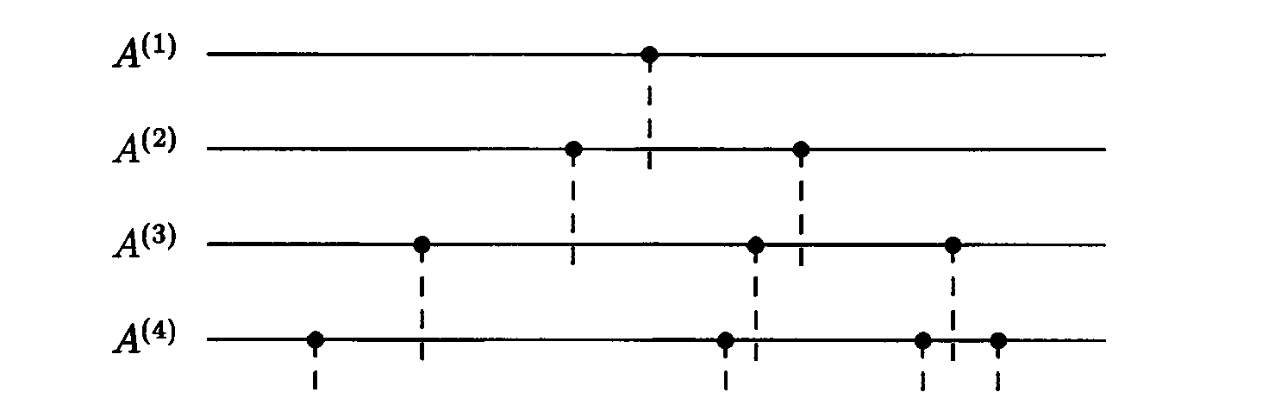
\includegraphics[width=0.8\textwidth]{figures/30-1.png}
    \caption{Illusion of the strict eigenvalue interlace property from the principal submatrice $ \{A^{(j)}\}  $ of an irreducible tridagonal real symmetric matrix $ A $. The eigenvalues of $ A^{(k)} $ interlace those of $ A^{(k+1)} $. The bisection algorithm takes advantage of this property. }
\end{figure}
%────────────────────────────────────────

If there are zeros on the off-diagonal, then the eigenvalue problem can be deflated. Note that the eigenvalues of $ A^{(k)} $ are distinct. Let them be denoted by $ \lambda _1 ^{(k)}< \lambda _2^{(k)}< \cdots < \lambda _k^{(k)} $. The crucial property that makes bisection powerful is that these eigenvalues {\it strictly interlace}, satisfying the inequalities 
\[
    \lambda _j ^{(k+1)} < \lambda _j ^{(k)} < \lambda _{j+1}^{(k+1)}
\]
for $ k=1,2,\ldots ,m-1 $ and $ j=1,2,\ldots , k-1 $. This behavior is sketched in Figure 29.1.  

It is the interlacing property that makes it possible to count the exact number of eigenvalues of a matrix in a specified interval. For example, consider the $ 4\times 4 $ tridiagonal matrix 
\[
    A =\begin{bmatrix}[1] 
        1 & 1 &  &   \\
        1 & 0 & 1 &   \\
         & 1 & 2 &  1 \\
         &  & 1 &  -1 \\
    \end{bmatrix}. 
\] 
From the numbers 
\[
    \det (A^{(1)}) = 1, \quad \det (A^{(2)}) = -1, \quad \det (A^{(3)}) = -3, \quad \det (A^{(4)}) = 4, 
\]
We know that $ A^{( 1)} $ has no negative eigenvalues, $ A^{(2)} $ has one negative eigenvalue, $ A^{(3)} $ has one negative eigenvalue, and $ A^{(4)} $ has two negative eigenvalues. In general, for any symmetric tridiagonal $ A\in \RR^{m\times m} $, the number of negative eigenvalues is equal to the number of sign changes in the sequence 
\[
    1, \det (A^{(1)}), \det (A^{(2)}), \ldots , \det (A^{(m)}), 
\]
which is known as a \textbf{Sturm sequence}. By shifting $ A $ by a multiple of the identity, we can determine the number of eigenvalues in any interval $ [a,b) $: it is the number of eigenvalues in $ (-\infty, b) $ minus the number in $ (-\infty,a) $.  

One more observation completes the description of the bisection algorithm. Expanding $ \det (A^{(k)}) $ by minors, we have 
\[
    \det (A^{(k)}) = a_k \det (A^{(k-1)}) - b_{k-1}^2 \det (A^{(k-2)} ).        
\]
Introducing the shift by $ xI $ and writing $ p^{(k)}(x) = \det (A^{(k)}-xI) $, we get 
\begin{equation}
\label{eq: bisection induction formula }
        p^{(k)}(x) = (a_k -x) p^{(k-1)}(x) - b_{ k-1 } ^2 p^{(k-2)}(x). 
\end{equation}
We can define $ p^{(-1)}(x) = 0, p^{(0)}(x) = 1 $.  


By applying \eqref{eq: bisection induction formula } for a succession of values of $ x $ and counting sign changes along the way, the bisection algorithm locates eigenvalues in arbitrarily small intervals. The cost is $ O(m) $ flops for each evaluation of the sequence, hence $ O(m\log (\mep)) $ flops in total to find an eigenvalue to relative accuracy $ \mep $. If a small number of eigenvalues are needed, this is a distinct improvement over the $ O(m^{2} ) $ operation count for the QR algorithm. On a multiprocessor computer, multiple eigenvalues can be found independently on separate processors. 


\section{Divide-and-Conquer} 
The divide-and-conquer algorithm, based on a recursive subdivision of a symmetric tridiagonal eigenvalue problem into problems of smaller dimension, represents the most important advance in matrix eigenvalue algorithms since the 1960s. First introduced by Cuppen in 1981, this methods is more than twice as fast as the QR algorithm if eigenvectors as well as eigenvalues are required.  

We shall give just the essential idea, omitting all details. But the reader is warned that in this area, the details are particularly important, for the algorithm is not fully stable unless they are gotten right--a matter that was not well understood for a decade after Cuppen's original paper. 

Let $ T\in \RR^{m} $ with $ m\ge 2 $ be symmetric, tridiagonal, and irreducible. Then $ \forall 1\le n<m,T$ can be split into submatrices as follows: 
%────────────────────────────────────────
\begin{figure}[H]
    \centering
    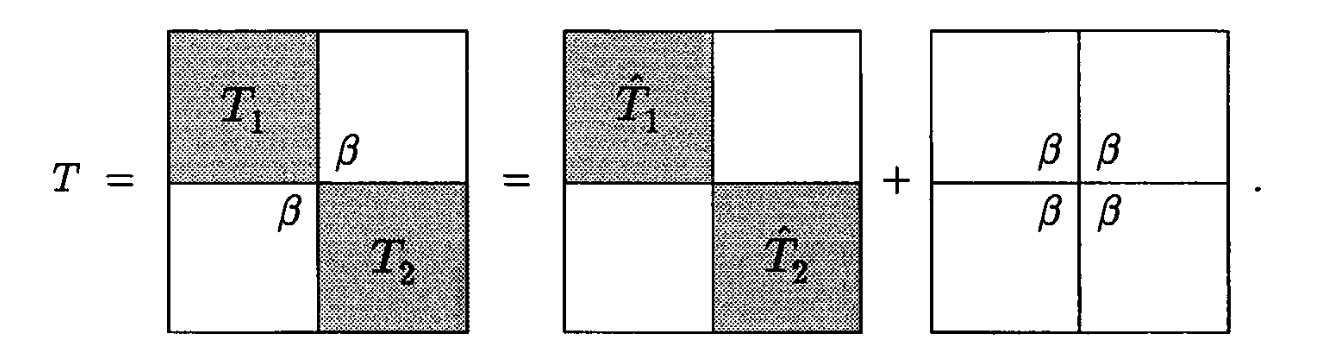
\includegraphics[width=0.8\textwidth]{figures/30-2.png}
\end{figure}
%────────────────────────────────────────  
where $ T_1 \in \RR^{n\times n}, T_2 \in \RR^{(m-n)\times (m-n)} $ and $\beta  = t_{n+1,n} = t_{n,n+1}\neq 0$.  Note that $(T_1)_{ nn } = (\hat T_1)_{nn} + \beta $ and $ (T_2)_{11} = ( \hat T_2 ) _{11} +\beta  $. Besides, the rightmost matrix has rank one.  In a word, a tridiagonal matrix can be written as the sum of a $ 2\times 2 $ block-diagonal matrix with tridiagonal blocks and a rank-one correction. 

The divide-and-conquer algorithm proceeds as follows. Split the $T$ with $n\approx \frac{m}{2}$. Suppose the eigenvalues of $ \hat T_1 $ and $ \hat T_2 $ are known. Since the correction  matrix is of rank one, a nonlinear but rapid calculation can be used to get from the eigenvalues of $ \hat T_1 $ and $ \hat T_2 $ to those of $ T $ itself. Now recurse on this idea, finding the eigenvalues of $ \hat T_1 $ and $ \hat T_2 $ by further subdivisions with rank-one corrections, and so on. In this manner an $ m \times  m $ eigenvalue problem is reduced to a set of $ 1\times 1 $ eigenvalue problems together with a collection of rank-one corrections. (In practice, for maximal efficiency, it's customary to switch to the QR algorithm when the submatrices are of sufficiently small dimension rather than to carry the recursion all the way.). 

In this process there is one key mathematical point. If the eigenvalues of $ \hat T_1 $ and $ \hat T_2 $ are known, how can those of $ T$ be found? Assume 
\[
    \hat T_1 = Q_1 D_1 Q_1^\top , \quad \hat T_2 = Q_2 D_2 Q_2^\top  
\]
have been computed. Then it follows that 
\begin{equation}
\label{eq: conquer step }
        T = \begin{bmatrix}[] 
        Q_1 &   \\
         &  Q_2 \\
    \end{bmatrix} \left( \begin{bmatrix}[] 
        D_1 &   \\
         &  D_2 \\
    \end{bmatrix} + \beta zz^\top    \right) \begin{bmatrix}[] 
        Q_1^\top  &   \\
         &  Q_2^\top  \\
    \end{bmatrix}  
\end{equation}

with $ z^\top  = ( q_1^\top ,q_2^\top  ) ,$ where $ q_1^\top  $ is the last row of $ Q_1 $ and $ Q_2^\top  $ is the first row of $ Q_2 $.  Hence, we have have to figure the eigenvalues of a diagonal matrix plus a rank-one correction.  

We show how this is done. We consider a simplified example. Suppose we wish to find the eigenvalues of $ D + ww^\top  $, where $ D\in \RR^{m\times m} $ is a diagonal matrix with distinct diagonal entries $ \{d_j\}  $ and $ w\in\RR^{m} $ is a vector. Here, we assume $ w_j\neq 0 $ for all $ j $, for otherwise, the problem is reducible. Then the eigenvalues of $ D+ww^\top  $ are the roots of the rational function
\[
    f(\lambda ) = 1+ \sum_{j=1}^{m} \frac{w_j^{2} }{d_j-\lambda },
\]
as illustrated in Figure 29.2. 

%────────────────────────────────────────
\begin{figure}[H]
    \centering
    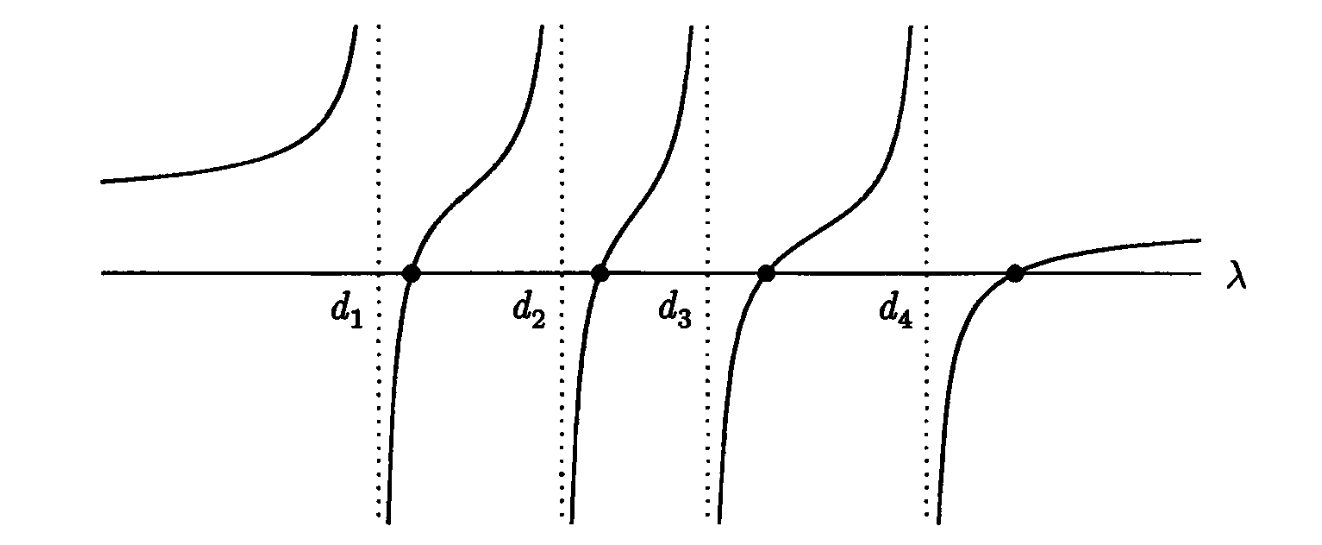
\includegraphics[width=0.8\textwidth]{figures/30-3.png}
    \caption{Plot of the function $ f(\lambda)$ for a problem of dimension $ 4 $. The poles of $ f(\lambda ) $ are the eigenvalues $ \{d_j\}  $ of $ D $, and the roots of $ f(\lambda ) $ are the eigenvalues of $ D+ww^\top  $. The rapid determination of these roots is the basis of each recursive step of the divide-and-conquer algorithm. }
\end{figure}
%────────────────────────────────────────

This assertion can be justified by that 
\[
    (D+ww^\top ) q = \lambda q \Rightarrow (D - \lambda I)q + w(w^\top q) =0 \Rightarrow q+(D-\lambda I)^{-1} w(w^\top q) =0 \Rightarrow w^\top q + w^\top (D-\lambda I)^{-1}  w(w^\top q) = 0. 
\]
Hence, we have $ f(\lambda ) (w^\top q) =0 $, in which $ w^\top q $ must be nonzero.  Hence, if $ q $ is an eigenvector of $ D+ww^\top  $ with eigenvalue $ \lambda  $, then $ f(\lambda )=0 $.  The equation $ f(\lambda ) $ is known as the \textbf{secular equation}.

At each step of the divide-and-conquer algorithm, the roots are found by Newton's method. Only $ O(1) $ iterations are required for each root (or $ O(\log(|\log(\mep)|)) $ iterations if $ \mep $ is viewed as a variable), making the operation count $ O(m) $ flops per root for an $ m\times m $ matrix, or $ O(m^{2} ) $ all tother. If we image a recursion in which a matrix of  dimension $ m $ is split exactly in half at each step, the total operation count for finding eigenvalues of a tridiagonal matrix by the divide-and-conquer algorithm becomes
\begin{equation}
\label{eq: cost of conquer}
        O\left( m^{2}  + \left( \frac{m}{2} \right) ^{2}  + 4\left( \frac{m}{4} \right) ^{2}  +\cdots + m  \left( \frac{m}{m} \right) ^{2}  \right) ,
\end{equation}

a series which converges to $ O(m^{2} ) $. Thus the operation count would appear to be of the same order $ O(m^{2} ) $ as for the QR algorithm.  


So far, it is not clear why the divide-and-conquer algorithm is advantageous. Since the reduction of a full matrix to tridiagonal form requires $ \frac{4m^3}{3} $ flops, it would seeme that any improvement in the $ O(m^{2} ) $ operation count for diagonalization of that tridiagonal matrix is hardly important. However, the economics change if one is computing eigenvectors as well as eigenvalues. Now, Phase 1 requires $ \frac{8m^3}{3} $ but Phase 2 also requires $ O(m^{3}) $ flops--for the QR algorithm, $ \approx 6m^{3} $. The divide-and-conquer algorithm reduces this figure, ultimately because its nonlinear iterations involve just the scalar function, not the orthogonal matrices $ Q_j $, whereas the QR algorithm must manipulate matrices $ Q_j $ at every iterative step.  

An operation count reveals the following. The $ O(m^{3}) $ part of the divide-and-conquer computation is the multiplication by $ Q_j $ and $ Q_j^\top  $ in \eqref{eq: conquer step }. The total operation count, summed over all steps of recursion is $ \frac{4m^3}{3} $ flops a great improvement over $ \approx 6m^{3} $ flops. Adding in the $ \frac{8m^3}{3} $flops for Phase 1 gives an improvement from $ \approx 9m^3 $ to $ 4m^3 $. 

Actually, the DC algorithm uusually does better, since for most matrices $ A $, many of the vectors $ z $ and matrices $ Q_j $ that arise in \eqref{eq: conquer step } turn out to be numerically sparse in the sense that many of their entries have relative magnitudes less than machine precision. This sparsity allows a process of numerical deflation, whereby successive tridiagonal eigenvalue problems are reduced to uncoupled problems of smaller dimensions. In typical cases, this reduces the Phase 2 operation count to an order less than $ m^{3} $ flops, reducing the operation count for Phase 1 and 2 combined to $ \frac{8m^3}{3} $. For eigenvalueus alone, the cost \eqref{eq: cost of conquer} becomes an overestimate and the Phase 2 operation count is reduced to an order lower than $ m^{2}  $ flops. The root of this fascinating phenomenon of deflation, which we shall not discuss further, is the fact that most of eigenvectors of most tridiagonal matrices are ``exponentially localized''--a fact that has related by physicists to the phenomenon that glass is transparent. 

We have spoken as if there is a single divide-and-conquer algorithm , but in fact, there are many variants. MOst complicated rank-one updates are often used for stability reasons, and rank-two updates are also sometimes used. Various methods are employed for finding the roots of $ f(\lambda ) $, and for large $ m $, the fastest way to carry out the multiplications by $ Q_j $ is via multipole expansions rather than the obvious algorithm. A high-quality implementation of a divide-and-conquer algorithm can be found in the LAPACK library.  